\section{ZenML}
De tweede tool waarvan een Proof of Concept gemaakt wordt is ZenML. Dit zal, in combinatie met MLFlow, gebruikt worden voor het lokaal uitvoeren van Machine Learning pipelines. Hierbij worden alle aanpassingen in de code van het framework vergeleken met de originele code van opdracht 3 van opleidingsonderdeel Machine Learning Operations.

\subsection{Installatie}
De installatie van ZenML gebeurt via de package manager \texttt{pip} en kan met het volgende commando geïnstalleerd worden.
\begin{minted}{bash}
    pip install zenml
\end{minted}
Er moet wel rekening gehouden worden dat ZenML alleen werkt met de Python versies 3.8, 3.9, 3.10 en 3.11.
Voor het lokaal uitvoeren van het ZenML dashboard moet er ook nog een extra package geïnstalleerd worden:
\begin{minted}{bash}
    pip install "zenml[server]"
\end{minted}

Nu de server geïnstalleerd is, kan deze worden opgestart met het volgende commando: 
\begin{minted}{bash}
    zenml up --blocking
\end{minted}
Er wordt een extra parameter \texttt{blocking} toegevoegd omdat Windows ZenML niet als achtergrondproces kan uitvoeren. Het is ook mogelijk om ZenML in een Docker-container uit te voeren met de parameter \texttt{docker}.

Na het opstarten van de server kan in de console het serveradres gevonden worden, zoals te zien is in de Figuur~\ref{fig:ZenMLServer}
\begin{figure}[h]
    \centering
    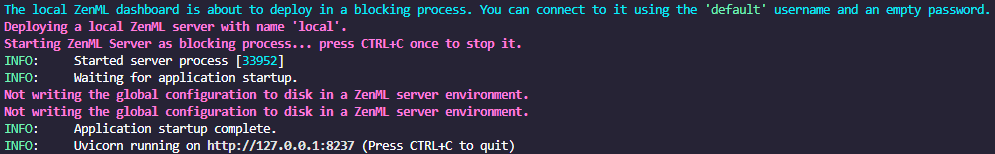
\includegraphics[width=0.9\linewidth]{graphics/ZenML_Server.PNG}
    \caption{ZenML server uitvoer na het opstarten}
    \label{fig:ZenMLServer}
\end{figure}
\subsection{Dashboard}
Wanneer er genavigeerd wordt naar het serveradres, zal er gevraagd worden om in te loggen. De inloggegevens zijn te zien bij het opstarten van de server in de console. Figuur~\ref{fig:ZenMLServer} toont dit ook aan. Hier kan gezien worden dat de gebruikersnaam \texttt{default} is en dat het wachtwoord leeg gelaten mag worden. Het inlogscherm ziet eruit zoals weergegeven in Figuur~\ref{fig:ZenML_Login}
\begin{figure}[h]
    \centering
    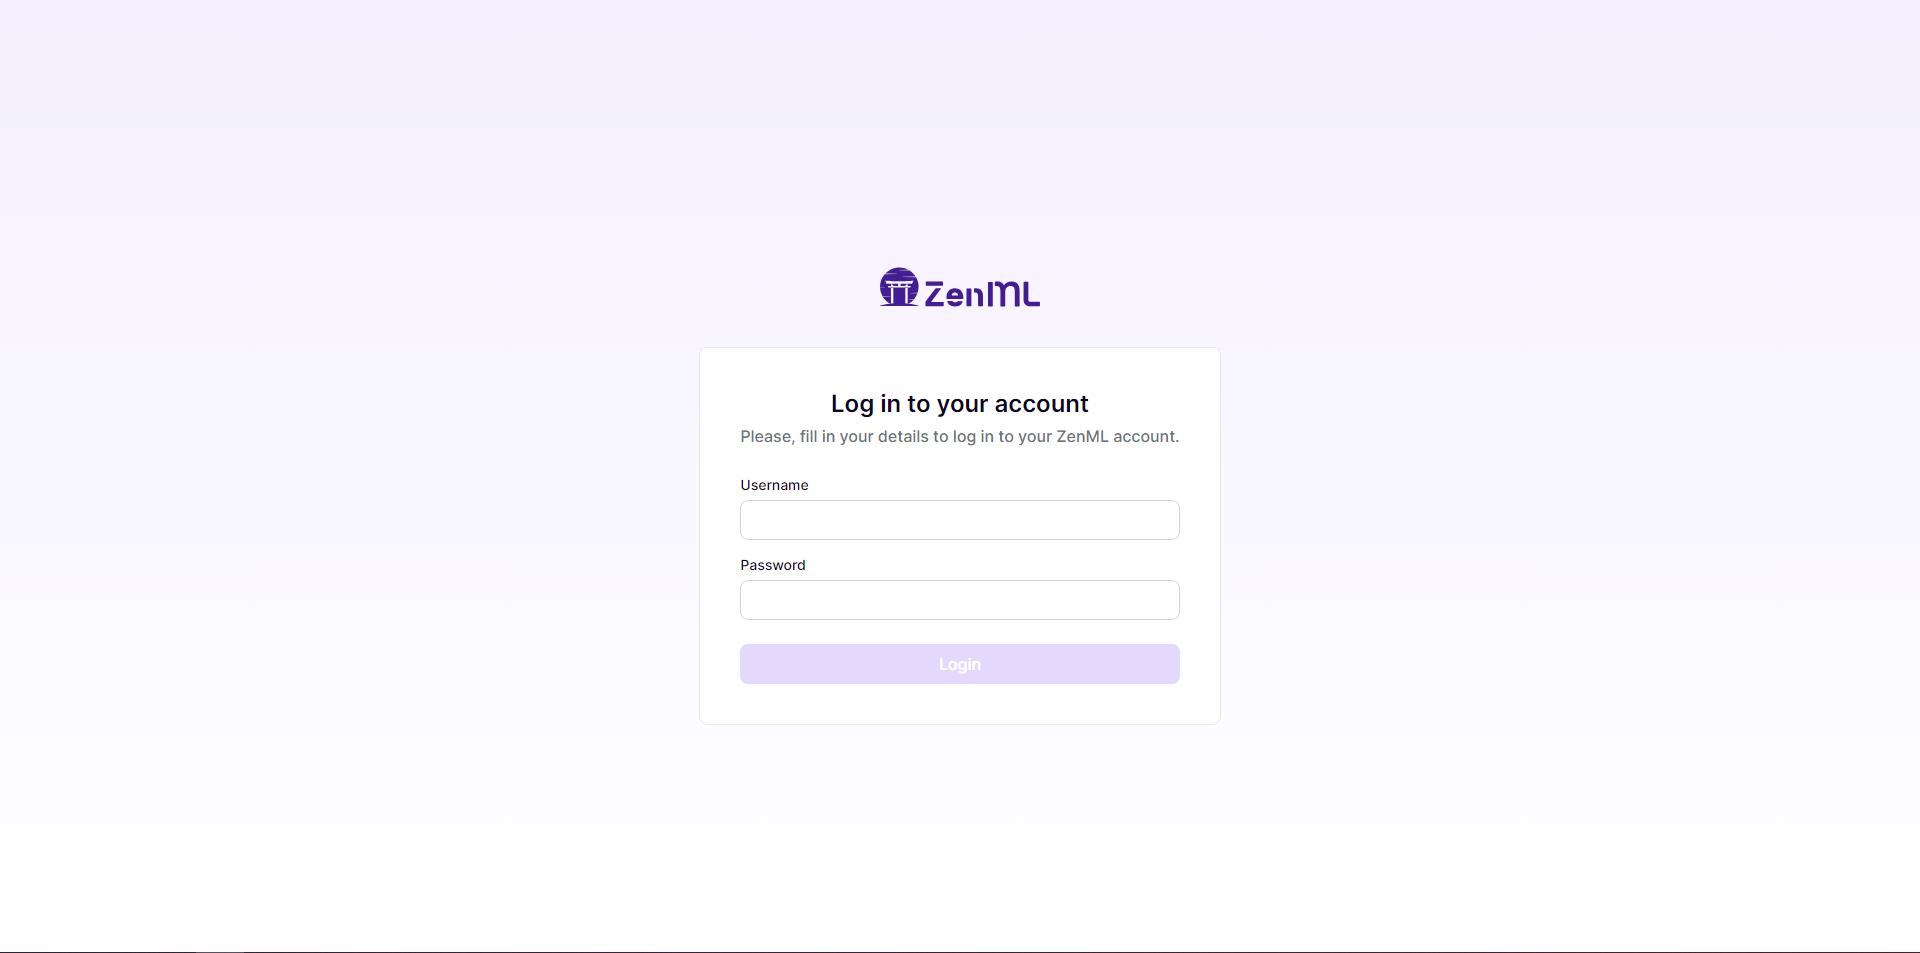
\includegraphics[width=0.9\linewidth]{graphics/ZenML_Login.PNG}
    \caption{ZenML authenticatie pagina}
    \label{fig:ZenML_Login}
\end{figure}
Na het inloggen wordt gevraagd om enkele basisgegevens, zoals je naam, e-mailadres, het gebruiksdoel van ZenML en hoe je ZenML hebt ontdekt. Het invullen van de naam en het e-mailadres is optioneel, maar de overige velden zijn verplicht.
Nu alles is ingevuld, wordt het dashboard getoond. Dit dashboard ziet eruit zoals op Figuur~\ref{fig:ZenML_Overview}
\begin{figure}[h]
    \centering
    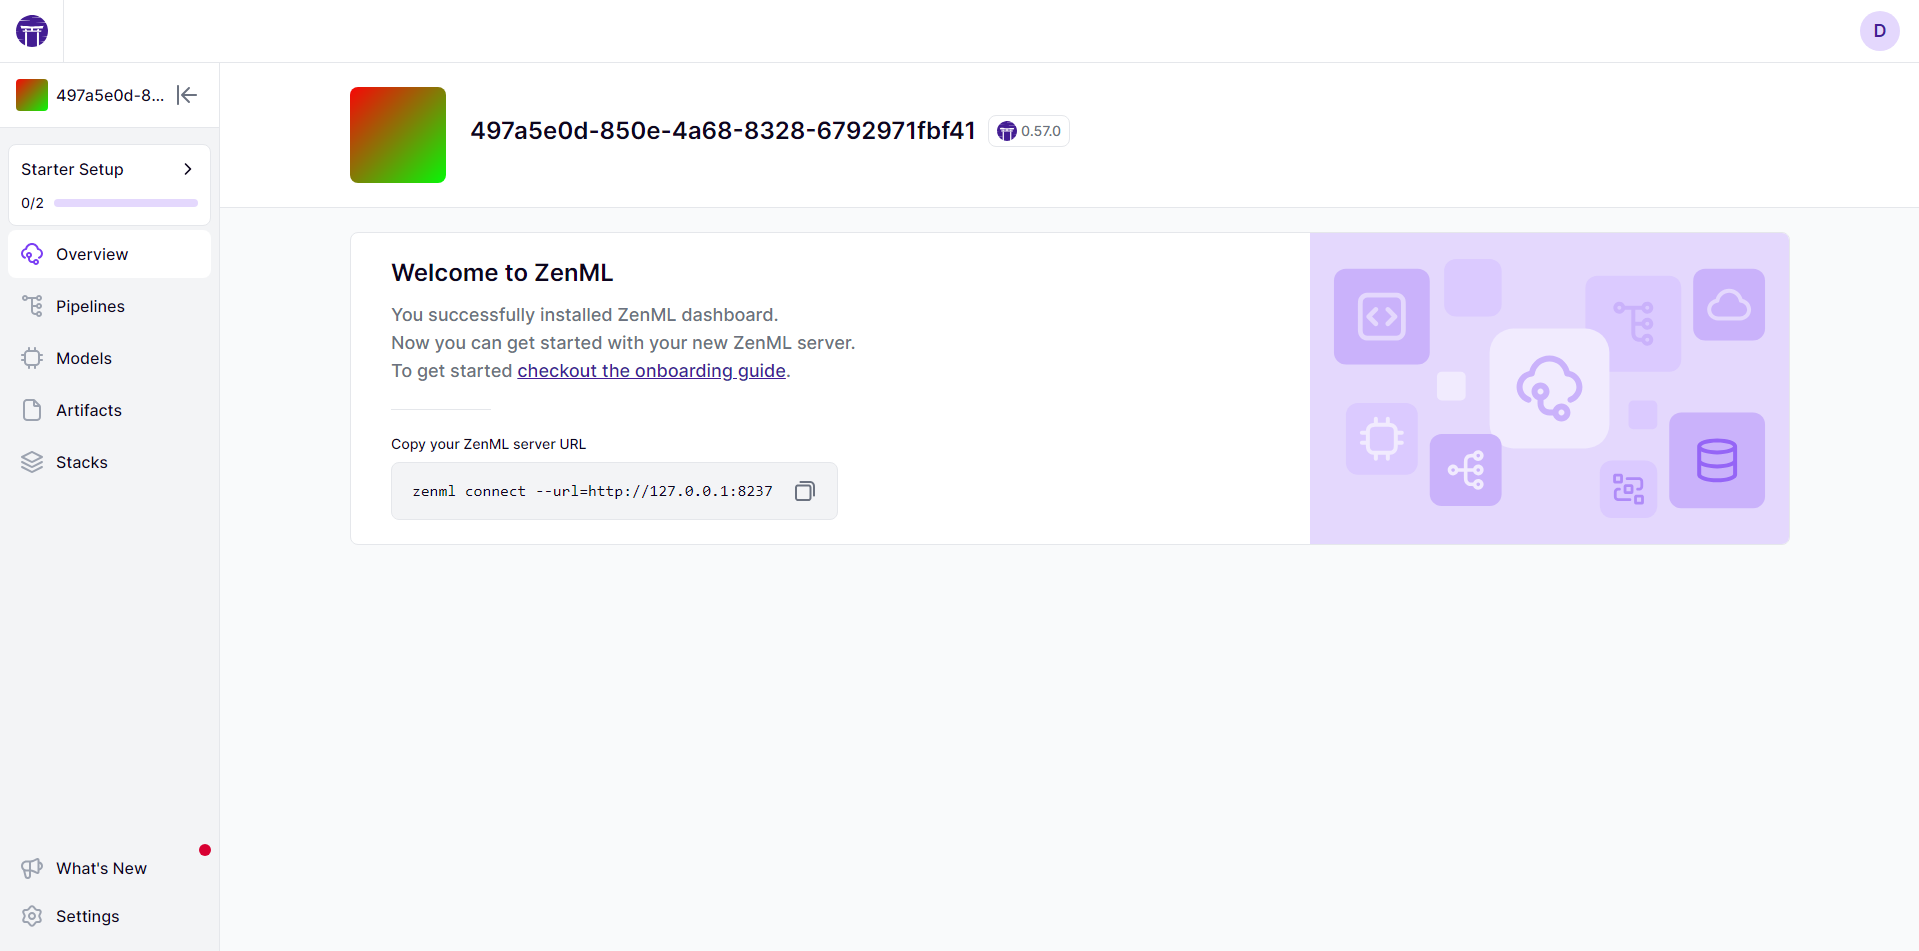
\includegraphics[width=0.9\linewidth]{graphics/ZenML_Overview.PNG}
    \caption{ZenML startpagina}
    \label{fig:ZenML_Overview}
\end{figure}

De functies die kunnen worden gezien zijn:

\begin{itemize}
    \item \textbf{Overview:} Geeft weer hoe je verbinding kan maken met de ZenML-server, zodat je meerdere computers aan één server kan koppelen.
    \item \textbf{Pipelines:} Geeft alle pipelines weer die werden of worden uitgevoerd.
    \item \textbf{Models:} Maakt het mogelijk omgetrainde Machine Learning modellen te beheren (dit is een ZenML Cloud optie en is betalend).
    \item \textbf{Artifacts:} De output van het training process wordt hier bijgehouden (dit is een ZenML Cloud optie en is betalend).
    \item \textbf{Stacks:} Hier kan verbinding gemaakt worden met verschillede integraties zoals Discord, Azure, Docker, Kubernetes\ldots
    \item \textbf{Settings:} Hier wordt alle gevoelige informatie bijgehouden, zoals wachtwoorden en API keys, en ook GitHub-repositories.
\end{itemize}

Deze Proof of Concept zal gebruik maken van de \textit{Pipelines} pagina op het dashboard.

\subsection{Uitvoering}
ZenML werkt met decorators. Dit zorgt ervoor dat bestaande Python-functies eenvoudig kunnen worden omgezet naar het ZenML framework. De twee decorators \texttt{@step} en \texttt{@pipeline} werden eerder in de Sectie~\ref{subsec:ZenML} besproken. Deze maken het mogelijk om bestaande Python functies om te zetten naar het ZenML framework.

Origineel bevatte het preprocessingsgedeelte zowel het downloaden als het verwerken van de afbeeldingen. Voor gebruik in ZenML is dit echter opgesplitst in twee aparte stappen: het downloaden en het verwerken van de afbeeldingen gebeurt nu afzonderlijk. Ook bij het maken van het model wordt het model eerst gebouwd en pas daarna getraind. In de originele code gebeurde dit in één functie.
De volledige code van de pipeline is te vinden in de GitHub-repository\footnote{\url{https://github.com/casperaudenaert/BP/tree/main/PoC/ZenML}} van deze Proof of Concept.

Alle functies werden een \texttt{step}. Dit werd gedaan door de decorators voor de functie te plaatsen. Uiteindelijk worden dan alle \texttt{steps} samengevoegd in één pipeline dit word aan de hand van de \texttt{pipeline} decorator gedefinieerd.
\subsection{Pipeline}
De pipeline in ZenML is een functie waarin alle taken en steps achter elkaar worden uitgevoerd. De pipeline ziet er als volgt uit:
\begin{minted}[frame=lines,breaklines,linenos]{python}
@pipeline(enable_cache=False)
def main():
    tracking_uri = "http://127.0.0.1:8080"
    model_name = "PoC"
    mlflow.set_tracking_uri(tracking_uri)
    mlflow.set_experiment(model_name)
    download(id="download")
    build_model(id="build",after="download")
    train(id="train",after="build")
    eval(id="eval",after="train")
\end{minted}
Deze code stelt eerst het juiste tracking adres voor MLflow in, alsook de modelnaam. Hierna worden alle functies achter elkaar uitgevoerd en kunnen deze dan ook in de dashboard gezien worden.

Elke \textit{step} heeft in dit geval een \textit{id}, wat ervoor zorgt dat de functies gemakkelijk in ZenML kunnen worden gebruikt. Dit is bijvoorbeeld handig voor de parameter \textit{after}, die ervoor zorgt dat een functie pas wordt uitgevoerd nadat de vorige functie is voltooid.

Alle \textit{steps} worden uitgevoerd in een \texttt{@pipeline} die nog een extra parameter \texttt{enable\_cache:} heeft. Deze parameter zorgt ervoor dat de functies die al zijn uitgevoerd in de cache worden opgeslagen, waardoor de volgende uitvoering sneller kan plaatsvinden.

Na het uitvoeren van de flow wordt deze flow gevisualiseerd in de webinterface van ZenML. Figuur~\ref{fig:ZenML_Pipeline_Flow} toont hoe deze pagina in ZenML eruit ziet.
\begin{figure}[h]
    \centering
    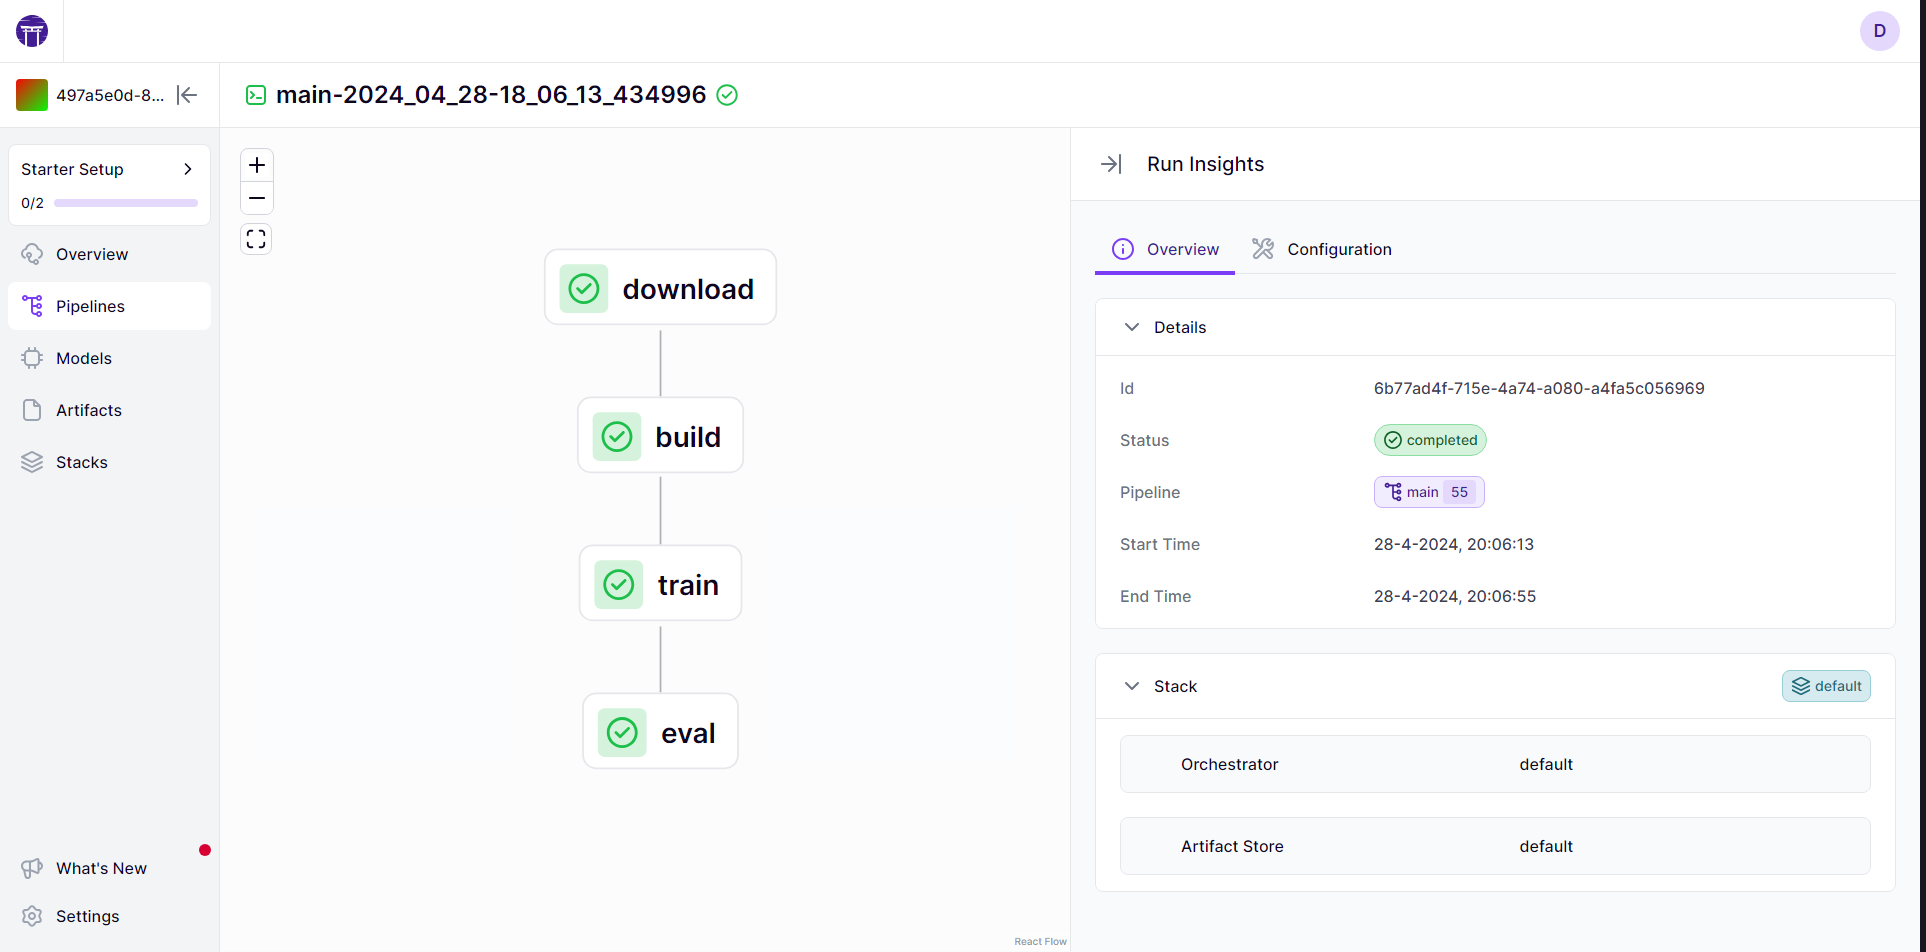
\includegraphics[width=0.9\linewidth]{graphics/ZenML_Pipeline_Flow.PNG}
    \caption{ZenML pipeline flow}
    \label{fig:ZenML_Pipeline_Flow}
\end{figure}
\subsection{Problemen}
Tijdens het uitvoeren van de Proof of Concept zijn er enkele problemen opgedoken.

Het eerste probleem was dat ZenML verschillende datatypes niet ondersteunt als parameters voor \textit{steps}, waardoor het model niet kon worden doorgegeven aan de volgende functie. Om dit op te lossen, werd het model lokaal opgeslagen en vervolgens in elke opeenvolgende functie opnieuw ingelezen.

Het tweede probleem was dat ZenML tijdens het opbouwen van deze Proof of Concept het hele dashboard had geüpdatet. Hierdoor is alles veranderd en zijn bepaalde functionaliteiten niet meer up-to-date met de documentatie van ZenML.

Het derde probleem was dat ZenML oudere versies van libraries gebruikte, wat tot conflicten leidde. Daarom werd voor alle Proof of Concepts een virtuele omgeving opgezet.

Het laatste probleem is dat ZenML de \textit{steps} niet in de volgorde uitvoert zoals ze in de \textit{pipeline} staan. Daarom moeten de \textit{steps} een \textit{id} krijgen, en de \textit{steps} die pas na een bepaalde \textit{step} kunnen worden uitgevoerd, moeten de parameter \textit{after} krijgen.
\subsection{Cloud}
ZenML heeft een concept genaamd \textit{Stacks}. Recentelijk is ZenML geüpgraded naar versie 0.57.0, waardoor het hele dashboard is vernieuwd en nog in ontwikkeling is. Deze pagina is dus nog niet beschikbaar, maar de functionaliteit kan al worden gebruikt via de command-line-interface (CLI).
Met Stacks is het mogelijk om verbinding te maken met verschillende integraties zoals AWS en Azure. Het unieke aspect van Stacks is dat verschillende onderdelen van de pipeline op verschillende platformen kunnen worden uitgevoerd. Bijvoorbeeld, het preprocessing kan plaatsvinden op Kubeflow, het trainen van het model op AWS, en het deployen van het model op Azure. Dit wordt mogelijk gemaakt door ZenML en vereenvoudigt het verbinden van verschillende integraties met elkaar.

Om een ZenML pipeline uit te voeren op Kubeflow kan het volgende commando gebruikt worden:
\begin{minted}[breaklines]{bash}
    zenml orchestrator register ORCHESTRATOR_NAME --flavor=ORCHESTRATOR_FLAVOR
\end{minted}
Waarbij de volgende twee parameters moeten aangepast worden:
\begin{itemize}
    \item \texttt{ORCHESTRATOR\_NAME:} De naam van deze \textit{orchestrator}.
    \item \texttt{ORCHESTRATOR\_FLAVOR\footnote{\url{https://docs.zenml.io/stacks-and-components/component-guide/orchestrators}}:} De integratie die wordt gebruikt voor het uitvoeren van de pipeline, zoals Azure of AWS.
\end{itemize}

